\hypertarget{_collision_object_8cpp}{}\section{C\+:/\+H\+A\+L/\+P\+G関係/03\+\_\+作成プログラム/03\+\_\+\+H\+A\+L授業/就職作品/\+Project/source/04\+\_\+\+Tool/\+Component/\+Base/\+Collision\+Base/\+Collision\+Object/\+Collision\+Object.cpp ファイル}
\label{_collision_object_8cpp}\index{C\+:/\+H\+A\+L/\+P\+G関係/03\+\_\+作成プログラム/03\+\_\+\+H\+A\+L授業/就職作品/\+Project/source/04\+\_\+\+Tool/\+Component/\+Base/\+Collision\+Base/\+Collision\+Object/\+Collision\+Object.\+cpp@{C\+:/\+H\+A\+L/\+P\+G関係/03\+\_\+作成プログラム/03\+\_\+\+H\+A\+L授業/就職作品/\+Project/source/04\+\_\+\+Tool/\+Component/\+Base/\+Collision\+Base/\+Collision\+Object/\+Collision\+Object.\+cpp}}
{\ttfamily \#include \char`\"{}Collision\+Object.\+h\char`\"{}}\newline
{\ttfamily \#include $<$Safe\+Release/\+Safe\+Release.\+h$>$}\newline
Collision\+Object.\+cpp の依存先関係図\+:\nopagebreak
\begin{figure}[H]
\begin{center}
\leavevmode
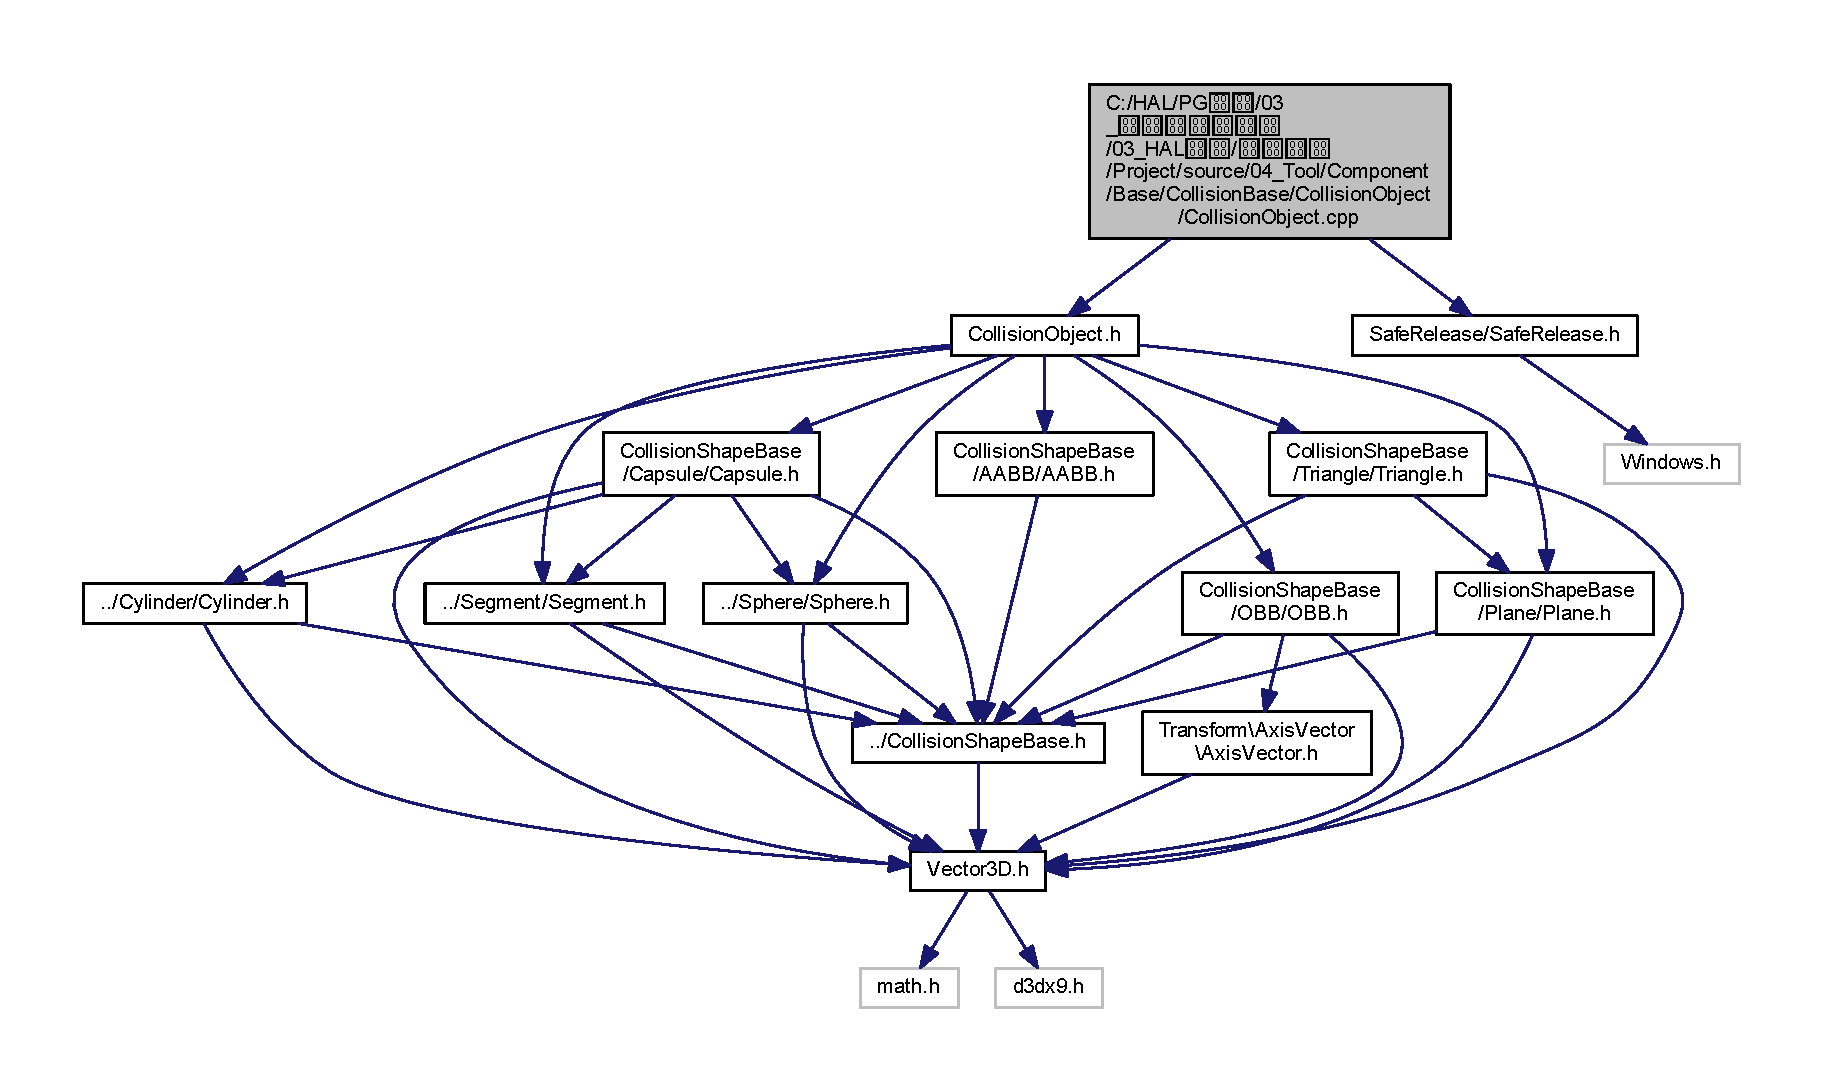
\includegraphics[width=350pt]{_collision_object_8cpp__incl}
\end{center}
\end{figure}
